\newpage
\section{JV editor (Steady state simulation editor)}
If you click on the JV editor icon in figure \ref{fig:ribbon_jv}, the JV editor window will open shown below in figure \ref{fig:jvcurveeditor}.

\begin{figure}[H]
\centering
\includegraphics[width=0.8\textwidth]{./images/sim_editors/ribbon_jv.png}
\caption{Opening the JV editor from the simulation editor ribbon.}
\label{fig:ribbon_jv}
\end{figure}

This window can be used to configure steady state simulations. It does not matter if you are running a current-voltage sweep on a solar cell or an OFET.  This plugin will steadily ramp the voltage from a start voltage to a stop voltage.  The voltage will be applied to the \emph{active} contact as defined in the \emph{contact editor}.  You can set the start voltage, stop voltage and step size.  Use \emph{JV voltage step multiplayer} to make the voltage step grow each step.  The default is 1.0, i.e. no growth.

\begin{figure}[H]
\centering
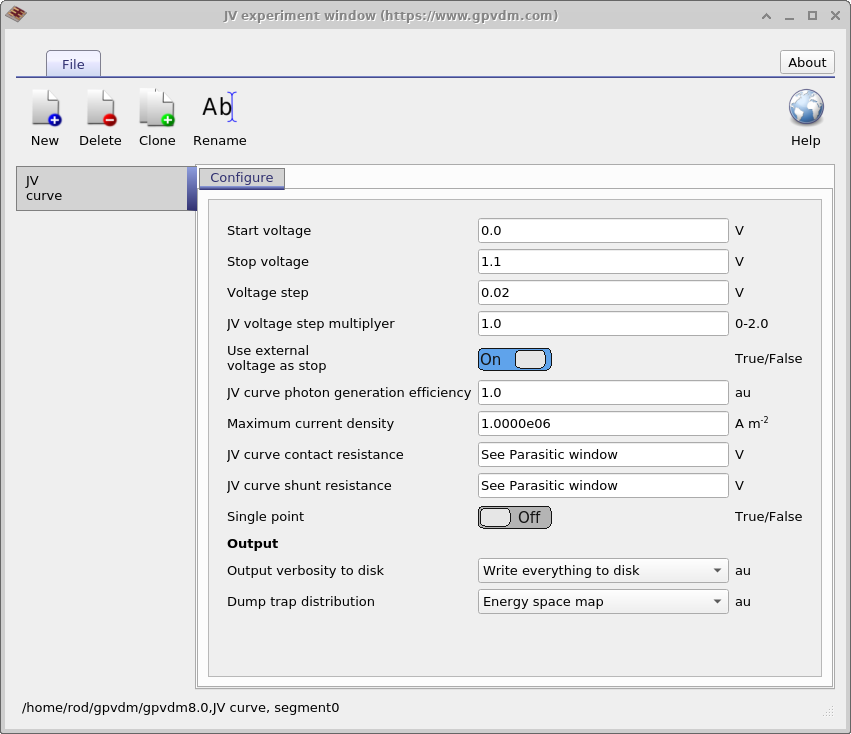
\includegraphics[width=0.7\textwidth,height=0.6\textwidth]{./images/sim_editors/jv_editor.png}
\caption{The JV editor editor window, use this to configure steady state simulations.}
\label{fig:jvcurveeditor}
\end{figure}

The files produced by the JV simulation mode are given in table \ref{tab:jv_output}.

\begin{table}[H]
\begin{center}
\begin{tabular}{ |c|c|c| } 
 \hline
	File name 			& 	Description  \\ 
 \hline
	$jv.dat$ 			&	Current voltage curve \\ 
	$charge.dat$ 		&	voltage charge density\\ 
	$k.csv$ 			&	Recombination constant k\\ 
	$sim\_info.dat$ 	&	Calculated $V_{oc}$, $J_{sc}$ etc.. see \ref{sec:siminfo}   \\

 \hline
\end{tabular}
\caption{Files produced by the JV simulation}
\label{tab:jv_output}
\end{center}
\end{table}


